\chapter{Estudo de Caso}\label{case_study}

Este capítulo apresenta dois estudos de caso para verificar a aplicabilidade da abordagem proposta na modelagem de interesses de uma aplicação. Os
estudos de caso são baseados no sistema para gerenciamento de hotel proposto por Jacobson \cite{Jacobson:2004:ASD:1062430}. Este exemplo possibilita a
modelagem de importantes funcionalidades de aspectos e foi utilizado para validar a abordagem de Jacobson. Os casos de uso tratados pelos
estudos de caso são: reserva de quartos, tratamento de uma lista de espera para clientes, registro de mensagens, \textit{check-out} de clientes e o
acúmulo de pontos em um programa de fidelidade. 

Os estudos de caso tratam da composição automática de modelos comportamentais, isto é, da composição de diagramas de sequência. O algoritmo de
composição para diagramas de sequência utiliza estereótipos e valores rotulados dos diagramas de classe. Por este motivo, modela-se também a
estrutura dos interesses de cada estudo de caso. Diagramas de sequência são utilizados para representar o comportamento dos interesses núcleo e
entrecortantes, usando o perfil UML e o processo proposto por esta abordagem. A modelagem de interesses usando diagramas comportamentais da UML 
fornece subsídios para realizar a troca de visões, a qual permite uma melhor compreensão de aplicações orientadas a aspectos, visualizando o efeito 
dos aspectos no sistema. O diagrama de classes é utilizado para modelar a estrutura dos interesses núcleo e entrecortantes.

A próxima seção apresenta o primeiro estudo de caso, que trata da composição de dois interesses entrecortantes (registro de mensagens e adição de
clientes em uma lista de espera) com um interesse núcleo para reserva de quartos. O segundo estudo de caso especifica a composição de um interesse
para acúmulo de pontos em um programa de fidelidade e o interesse de registro de mensagens com um interesse núcleo para realizar o \textit{check-out}
de clientes.

\section{Estudo de Caso: Reserva de Quarto, Registro de Mensagens e Lista de Espera}

O primeiro estudo de caso envolve três interesses do sistema:

\begin{itemize}
  \item \textbf{Reserva de Quartos:} Um cliente pode reservar um quarto, se o mesmo estiver disponível.
  \item \textbf{Registro de Mensagens:} O sistema registra as mensagens executadas em determinados componentes.
  \item \textbf{Lista de Espera:} Um cliente pode ser colocado em uma lista de espera quando um quarto não estiver disponível para reserva imediata.
\end{itemize}

  \begin{figure}[!h]
	\centering
	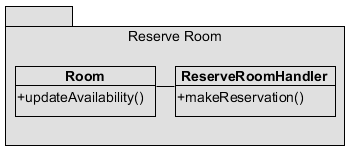
\includegraphics{img/case_study_structural_reserve_room.png}
	\caption{Modelagem estrutural: reserva de quarto}\label{fig:case_study_structural_reserve_room}
  \end{figure}

A modelagem de um interesse começa com a criação de um diagrama de classes que representa a sua estrutura. As classes e os aspectos que
representam o interesse ficam agrupadas dentro de um pacote da UML. Se o interesse for do tipo entrecortante, este pacote é marcado com o estereótipo
\textit{CrosscuttingConcern}. No caso do interesse ser do tipo núcleo, o pacote não é estereotipado. O diagrama de classes da figura
\ref{fig:case_study_structural_reserve_room} representa a estrutura do interesse para reserva de quartos. A modelagem estrutural do interesse para 
reserva de quarto contém a classe \textit{Room} com o método \textit{updateAvailability()} para atualizar a disponibilidade de um quarto. Este
interesse também tem a classe \textit{ReserveRoomHandler} com o método \textit{makeReservation()}, responsável por realizar a reserva de um quarto.

  \begin{figure}[!h]
	\centering
	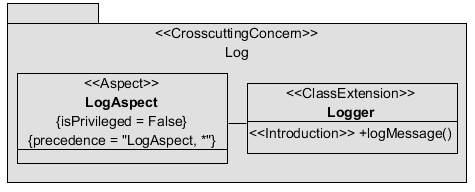
\includegraphics{img/case_study_structural_log.png}
	\caption{Modelagem estrutural: registro de mensagens}\label{fig:case_study_structural_log}
  \end{figure}

  \begin{figure}[!h]
	\centering
	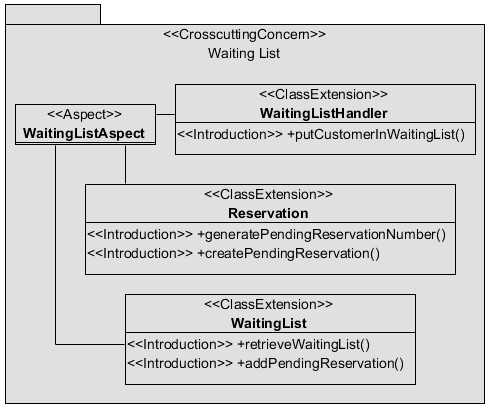
\includegraphics{img/case_study_structural_waiting_list.png}
	\caption{Modelagem estrutural: lista de espera}\label{fig:case_study_structural_waiting_list}
  \end{figure}

O segundo interesse modelado é o interesse entrecortante para registro de mensagens. Este interesse impacta vários componentes do sistema e é
marcado com o estereótipo \textit{CrosscuttingConcern}, para representar que o mesmo é entrecortante. A figura \ref{fig:case_study_structural_log}
apresenta a modelagem deste interesse. O interesse contém a classe \textit{Logger}, responsável por registrar as mensagens através do método
\textit{log()}. A classe \textit{Logger} é marcada com o estereótipo \textit{ClassExtension}, pois é uma nova classe no sistema. O método
\textit{log()} é estereotipado com \textit{Introduction}, pois é um método que está sendo inserido pelo interesse entrecortante para registro de mensagens. 
O aspecto \textit{LogAspect} é o aspecto que define os pontos de corte e avisos modelados nos diagramas de máquina de estados e nos digramas de
sequência. Existe uma associação entre o aspecto \textit{LogAspect} e a classe \textit{Logger}, pois o aspecto é o componente responsável por introduzir esta 
nova classe no sistema. Observa-se a presença do valor rotulado \textit{precedence} com o texto \textit{LogAspect, *}. Esta especificação define que o
aspecto para registro de mensagens tem precedência perante todos os outros aspectos do sistema (símbolo *), isto é, as mensagens deste aspecto serão
inseridas antes de outros aspectos no caso de um aviso conflitante do tipo antes. O mesmo vale para os outros tipos de aviso.

O interesse para controle de uma lista de espera de clientes é representado na modelagem da figura \ref{fig:case_study_structural_waiting_list}. O
pacote com as classes que representam o interesse também é marcado com o estereótipo \textit{CrosscuttingConcern}. O aspecto \textit{WaitingListAspect} está
associado com as classes \textit{WaitingListHandler}, \textit{Reservation} e \textit{WaitingList}. Essas três classes são extensões a classes do
sistema e estão estereotipadas com \textit{ClassExtension}. A classe \textit{WaitingListHandler} é a responsável pelo controle da lista de espera, com
o método \textit{putCustomerInWaitingList()}, que adiciona um cliente na lista de espera. A classe \textit{Reservation} contém um método para criar
uma reserva (\textit{createPendingReservation()}) e outro método para gerar um número para esta reserva (\textit{generatePendingReservationNumber()}).
Finalmente, a classe \textit{WaitingList} contém os métodos \textit{retrieveWaitingList()}, para obter a lista de espera, e o método
\textit{addPendingReservation()} para adicionar uma reserva de um cliente. Todos os métodos pertencentes a estas classes estão estereotipados com
\textit{Introduction}, pois são introduções estruturais ao sistema de gerenciamento de hotel.

Após a modelagem da estrutura dos interesses, deve-se modelar o comportamento dos mesmos. A especificação do comportamento de um interesse núcleo
envolve apenas o diagrama de sequência. Já os interesses entrecortantes devem ser modelados com um diagrama de máquina de estados para representar
seus pontos de corte e um diagrama de sequência para representar a execução do comportamento do aspecto. Os pontos de corte definem quais pontos do
sistema serão estendidos. O comportamento de um aspecto é representado pelos avisos associados ao mesmo. O diagrama de sequência que representa o
comportamento de um aspecto, também representa a conexão entre a satisfação de um ponto de corte com a execução das mensagens do aviso de um aspecto.

  \begin{figure}[!h]
	\centering
	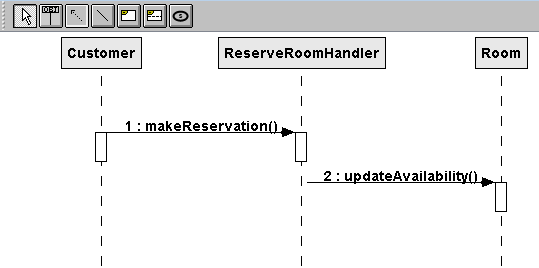
\includegraphics{img/case_study_behavioral_reserve_room.png}
	\caption{Diagrama de sequência: reserva de quarto}\label{fig:case_study_behavioral_reserve_room}
  \end{figure}

O primeiro diagrama de sequência é o que representa a troca de mensagens do interesse núcleo para reserva de quartos. O diagrama pode ser visualizado
na figura \ref{fig:case_study_behavioral_reserve_room}. Para realizar uma reserva de quarto, primeiramente realiza-se uma chamada ao método
\textit{makeReservation()} da classe \textit{ReserveRoomHandler} que é responsável por iniciar a reserva. Após esta chamada, executa-se o método
para verificar se o quarto está disponível. Se o quarto não estiver disponível, uma exceção é lançada no método \textit{updateAvailability()}, caso
contrário, a reserva é realizada e o cliente recebe um código de confirmação.
  
O interesse entrecortante para registro de mensagem contabiliza o número de requisições a um quarto. Para realizar este objetivo, define-se um ponto
de corte que captura qualquer chamada a classes do tipo \textit{Room}. Este ponto de corte é modelado usando o diagrama de máquina de estados da UML e 
pode ser visualizado na figura \ref{fig:case_study_behavioral_pointcut_log}. 

Com o ponto de corte especificado, cria-se o diagrama de sequência para representar a troca de mensagens entre objetos para realização do registro de
chamadas. O diagrama pode ser visualizado na figura \ref{fig:case_study_behavioral_log} e contém o aspecto \textit{LogAspect} associado a primeira linha de vida do diagrama. De acordo com a
abordagem proposta, um aspecto no diagrama de sequência deve ter uma invariante de estado associada, a qual é o gatilho 
para começar a executar a sequência de mensagens do diagrama. No exemplo em questão, a invariante de estado \textit{RoomCall} está associada ao
aspecto \textit{LogAspect} e referencia o ponto de corte definido previamente no diagrama de máquina de estados. A semântica é que 
a sequência de mensagens só será executada quando o ponto de corte for satisfeito. A mensagem a ser executada
é uma chamada ao método \textit{log()} da classe \textit{Logger}. É importante observar o tipo de aviso, que é definido como um valor rotulado na
invariante de estado. O valor rotulado não está sendo mostrado no diagrama de sequência por configuração de visualização, já que por padrão os valores 
rotulados não são exibidos. A abordagem proposta suporta três tipos de aviso: antes, durante ou depois. Neste caso, o
tipo de aviso é depois, o que significa que o comportamento de registro de mensagens somente executará após a chamada a qualquer método da classe
\textit{Room}. O diagrama de sequência contém um fragmento combinado do tipo opcional, o qual define que o registro de mensagens executará se a
aplicação não estiver congelada. Uma aplicação está congelada quando está executando diretamente para o usuário e é considerada congelada no ambiente
de desenvolvimento.

  \begin{figure}
	\centering
	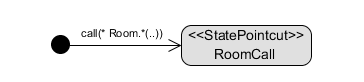
\includegraphics{img/case_study_behavioral_pointcut_log.png}
	\caption{Ponto de corte: registro de mensagens}\label{fig:case_study_behavioral_pointcut_log}
  \end{figure}
  
  \begin{figure}
	\centering
	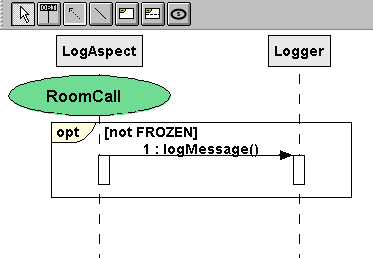
\includegraphics{img/case_study_behavioral_log.png}
	\caption{Aviso: registro de mensagens}\label{fig:case_study_behavioral_log}
  \end{figure}

O requisito para criação de uma lista de espera para clientes também é um interesse entrecortante. Este interesse adiciona um cliente a uma lista de
espera quando um quarto não está disponível. É necessário definir um ponto de corte que captura a tentativa de um cliente reservar um
quarto, mas o quarto está indisponível. A figura \ref{fig:case_study_behavioral_pointcut_waiting_list} representa um ponto de corte
para capturar as chamadas ao método \textit{updateAvailability()} da classe \textit{Room}, lançando a exceção \textit{NoRoomsAvailable}. Além da
definição de um ponto de corte, é necessário definir o comportamento de como um cliente é adicionado a lista de espera. O comportamento é modelado no
diagrama de sequência da figura \ref{fig:case_study_behavioral_waiting_list}. O diagrama tem o aspecto \textit{WaitingListAspect} associado a primeira 
linha de vida e uma sequência de mensagens para serem executadas quando o sistema lança uma exceção de quarto indisponível. Estas
mensagens são executadas depois do tratamento de exceção, pois o valor rotulado que define o tipo do aviso na invariante de estado é do tipo depois.

  \begin{figure}[tb]
	\centering
	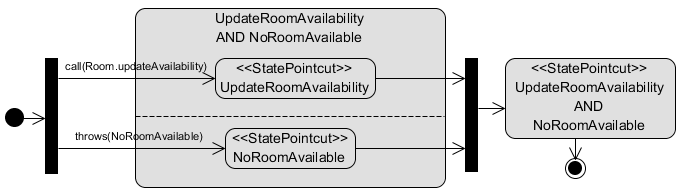
\includegraphics[scale=0.8]{img/case_study_behavioral_pointcut_waiting_list.png}
	\caption{Ponto de corte: controle de uma lista de espera}\label{fig:case_study_behavioral_pointcut_waiting_list}
  \end{figure}
  
  \begin{figure}
	\centering
	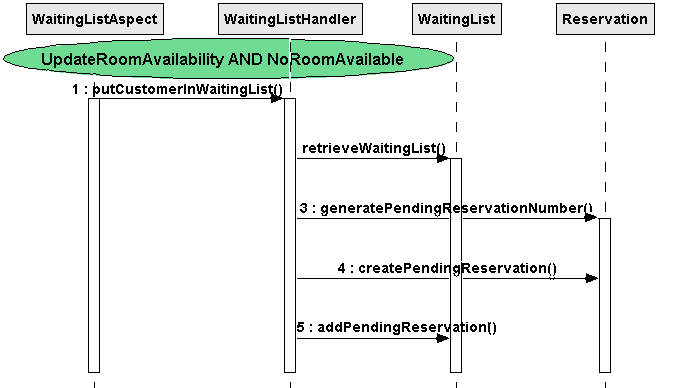
\includegraphics{img/case_study_behavioral_waiting_list.png}
	\caption{Aviso: controle de uma lista de espera}\label{fig:case_study_behavioral_waiting_list}
  \end{figure}
  
Depois da especificação estrutural e comportamental dos interesses núcleo e entrecortantes, o desenvolvedor pode intercambiar as visões do sistema,
selecionando quais interesses deseja visualizar em um mesmo diagrama. A ferramenta SEA/Aspect permite a seleção de um ou mais modelos para serem
compostos ao mesmo tempo. Uma configuração de composição é apresentada na figura \ref{fig:case_study_compound_2}, com os interesses para reserva de
quarto, registro de mensagens e tratamento da lista de espera. O diagrama composto exibe um seletor de modelos na parte de baixo da imagem, o qual 
permite a troca dos modelos que estão sendo compostos. As mensagens de diferentes
interesses são exibidas com cores diferentes, já que cada interesse tem uma cor associada. A mensagem do interesse de registro de mensagens
(\textit{log()}) está com o fundo vermelho. Já as mensagens do interesse para controle de uma lista de espera (\textit{putCustomerInWaitingList(),
retrieveWaitingList(), generatePendingReservationNumber(), createPendingReservation() e addPendingReservation()}) estão com o fundo verde. É
importante observar que o interesse para registro de mensagens tem precedência perante o interesse para controle de uma lista de espera, por isso a
mensagem \textit{log()} foi introduzida antes das mensagens do interesse de lista de espera no diagrama de sequência composto. A ordem de
precedência é definida pelo valor rotulado \textit{precedence}, configurado ao definir a estrutura do interesse de registo de mensagens na figura
\ref{fig:case_study_structural_log}.

\begin{landscape}
  \begin{figure*}[tb]
	\centering
	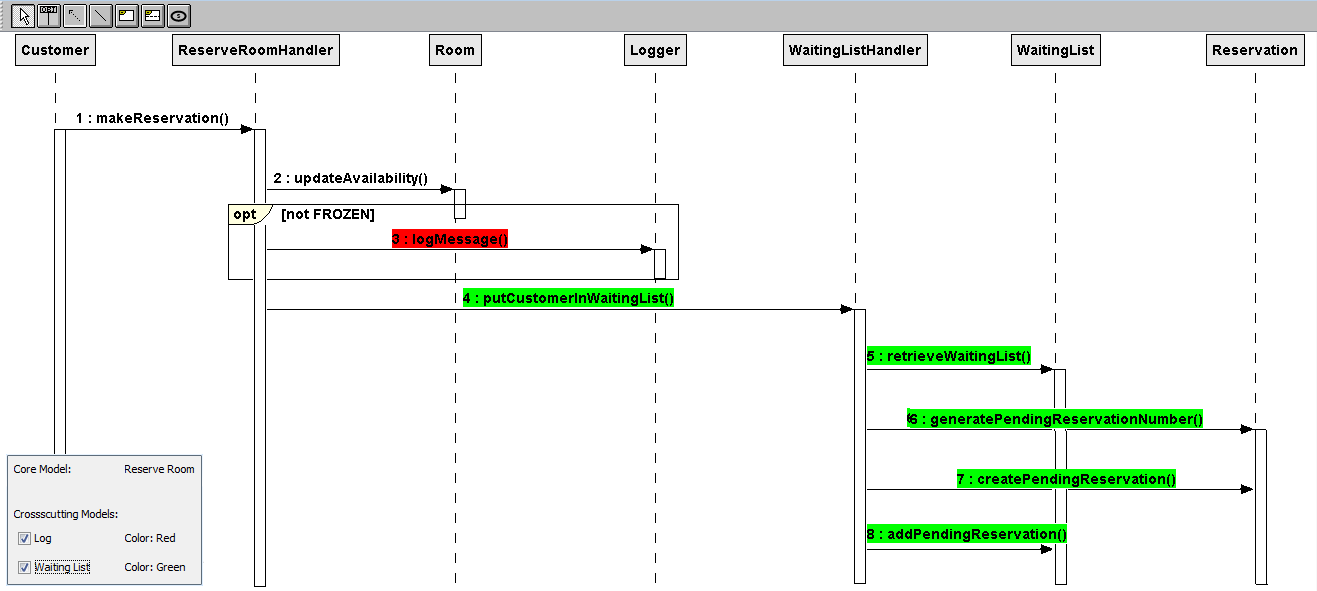
\includegraphics[scale=0.7]{img/case_study_compound_2.png}
	\caption{Estudo de caso: reserva de quarto composto com registro de mensagens e controle de lista de espera}\label{fig:case_study_compound_2}
  \end{figure*}
\end{landscape}
  
\section{Estudo de Caso: Check-out de Clientes, Registro de Mensagens e Programa de Fidelidade}

O segundo estudo de caso realiza a composição de três interesses. Um dos interesses envolvido é o de registro de mensagens, apresentado no estudo de
caso da seção anterior, e que não sera representado nesta seção. Os outros dois interesses são:

\begin{itemize}
  \item \textbf{Check-out de Clientes:} Um cliente do hotel pode realizar o check-out, após realizar o pagamento do quarto.
  \item \textbf{Programa de Fidelidade:} Após realizar o pagamento de um quarto, um cliente pode acumular pontos em um programa de fidelidade.
\end{itemize}

  \begin{figure}[!h]
	\centering
	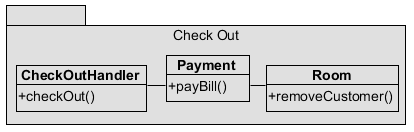
\includegraphics{img/case_study_structural_check_out.png}
	\caption{Modelagem estrutural: check-out de clientes}\label{fig:case_study_structural_check_out}
  \end{figure}

A especificação estrutural do interesse núcleo para \textit{check-out} de clientes pode ser visualizada na figura
\ref{fig:case_study_structural_check_out}. Este interesse contém a classe \textit{CheckOutHandler} que inicia a operação de \textit{check-out} através 
do método \textit{checkOut()}. A classe \textit{Payment} possui o método \textit{payBill()}, o qual permite realizar o pagamento de um quarto. A
classe \textit{Room} contém o método \textit{removeCustomer()}, para remover um cliente da lista de hóspedes do hotel. As classes do modelo estrutural
não estão estereotipados, pois representam um interesse núcleo do sistema.

  \begin{figure}[!h]
	\centering
	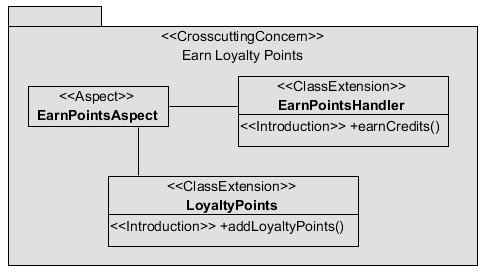
\includegraphics{img/case_study_structural_earn_points.png}
	\caption{Modelagem estrutural: acúmulo de pontos em programa de fidelidade}\label{fig:case_study_structural_earn_points}
  \end{figure}

O interesse para acúmulo de pontos em um programa de fidelidade tem sua modelagem estrutural apresentada na figura
\ref{fig:case_study_structural_earn_points}. Este interesse é do tipo entrecortante, pois estende o sistema adicionando um novo requisito que
permite o acúmulo de pontos após o pagamento de um quarto. O pacote que representa o interesse é estereotipado com o estereótipo
\textit{CrosscuttingConcern}. A modelagem estrutural contém duas classes: \textit{LoyaltyPoints} e \textit{EarnPointsHandler}, marcadas com o
estereótipo \textit{ClassExtension}. A primeira classe contém o método \textit{addLoyaltyPoints()}, que adiciona pontos ao saldo do programa de
fidelidade de um determinado cliente. A classe \textit{EarnPointsHandler} contém o método \textit{earnCredits()}, o qual controla a operação de
obtenção de pontos após o pagamento. Finalmente, o aspecto \textit{EarnPointsAspect} contém o estereótipo \textit{Aspect}, e introduz as mudanças
estruturais propostas pelas classes deste interesse.

  \begin{figure}[!h]
	\centering
	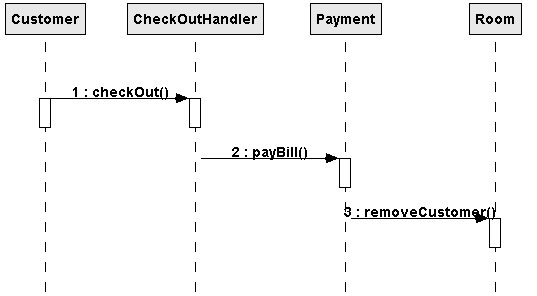
\includegraphics{img/case_study_behavioral_check_out.png}
	\caption{Diagrama de sequência: check-out de clientes}\label{fig:case_study_behavioral_check_out}
  \end{figure}

O diagrama de sequência que representa o comportamento do interesse para \textit{check-out} de clientes pode ser visualizado na figura
\ref{fig:case_study_behavioral_check_out}. A troca de mensagens do diagrama de sequência inicia quando o objeto \textit{CheckOutHandler} executa a
mensagem \textit{checkOut()}. Esta mensagem dispara a mensagem \textit{payBill()} para realizar o pagamento da conta do cliente. Após o pagamento da
conta, o cliente é removido da lista de clientes ativos através do método \textit{removeCustomer()} da classe \textit{Room}.

  \begin{figure}[!h]
	\centering
	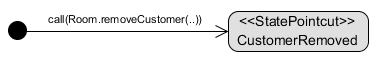
\includegraphics{img/case_study_behavioral_pointcut_loyalty_points.png}
	\caption{Ponto de corte: programa de fidelidad}\label{fig:case_study_behavioral_pointcut_loyalty_points}
  \end{figure}

A modelagem comportamental do interesse para acúmulo de pontos em um programa de fidelidade envolve a especificação de um ponto de corte e de um
aviso. O ponto de corte é especificado na figura \ref{fig:case_study_behavioral_pointcut_loyalty_points}. Este ponto de corte captura chamadas ao
método \textit{payBill()} da classe \textit{Payment}. O diagrama de sequência pode ser visualizado na figura
\ref{fig:case_study_behavioral_loyalty_points}. Este diagrama de sequência contém a invariante de estado \textit{BillPaid}, que está associada ao
aspecto \textit{EarnPointsAspect}. Esta invariante de estado contém o valor rotulado \textit{adviceType} com o valor \textit{after}. Isto significa que as
mensagens só serão executadas após a satisfação do estado \textit{BillPaid}. Após o disparo da invariante de estado, a classe
\textit{EarnPointsHandler} executa o método \textit{earnCredits()}. Este método dispara o método \textit{addLoyaltyPoints()} na classe
\textit{LoyalyPoints}, que adiciona pontos ao saldo de pontos do cliente no programa de fidelidade.
  
A figura \ref{fig:case_study_2_compound} apresenta a composição dos interesses para \textit{check-out} de clientes, registro de mensagens e acúmulo
de pontos em um programa de fidelidade. As mensagens do interesse para registro de mensagens estão com o fundo azul. Já as mensagens do programa de
fidelidade estão com o fundo amarelo. O interesse núcleo não teve suas mensagens modificadas. 
  
  \begin{figure}
	\centering
	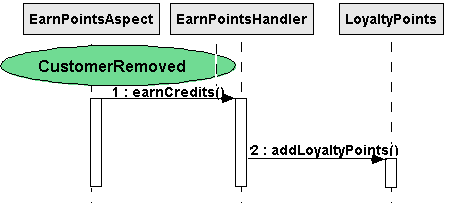
\includegraphics{img/case_study_behavioral_loyalty_points.png}
	\caption{Aviso: programa de fidelidade}\label{fig:case_study_behavioral_loyalty_points}
  \end{figure}

  \begin{landscape}
  \begin{figure*}[tb]
	\centering
	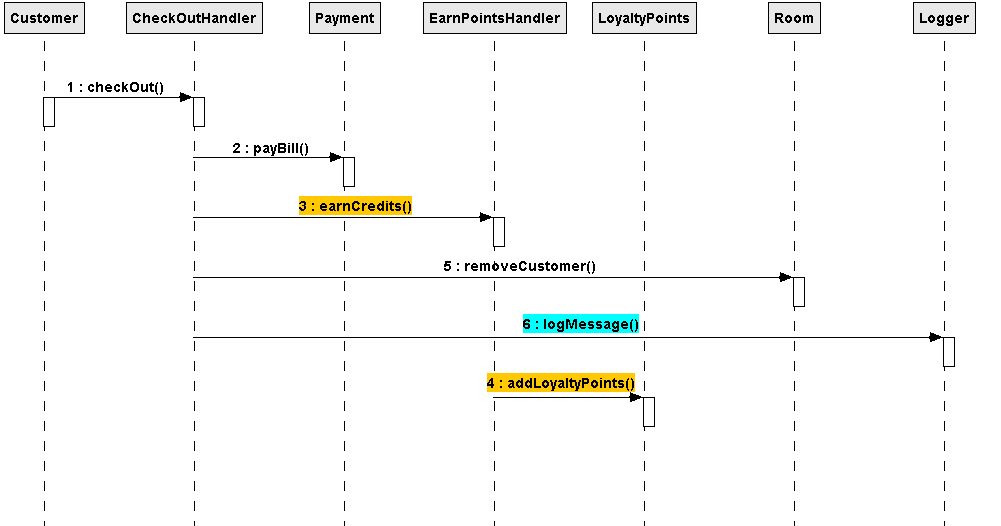
\includegraphics[scale=0.7]{img/case_study_2_compound.png}
	\caption{Estudo de caso: check-out de clientes composto com registro de mensagens e programa de fidelidade}\label{fig:case_study_2_compound}
  \end{figure*}
\end{landscape}
  
\section{Discussão}

A aplicação da abordagem em um estudo de caso mostra como a proposta para especificação e composição de aspectos facilita a compreensão de
sistemas orientados a aspectos, permitindo a alternância de visões, visualizando somente os interesses núcleo ou uma composição entre interesses núcleo e entrecortantes, 
sem esforço do desenvolvedor. Os modelos compostos mostram o efeito dos aspectos em um sistema, com cada aspecto diferenciado por uma única cor que o
representa. A ferramenta SEA/Aspect permite a separação de interesses nas primeiras fases de desenvolvimento, o que é um dos objetivos das abordagens para modelagem
de sistemas orientados a aspectos.
